

\textcolor{secundario}{METODOLOG\'IAS DE VALUACI\'ON FINANCIERA}. En vista de lo anterior, de conformidad con el marco jurídico señalado en el \autoref{cap:3} de este informe, se aplicaron las siguientes metodologías para ser utilizadas en la valuación del deterioro y lucro cesante marcario; derivado de los hechos mencionados en el antecedente de este capítulo:\\

\begin{figure}[H]
\centering
\caption{Metodolog\'ias de Valuaci\'on de Negocios m\'as utilizadas\label{fig:metodologias}}
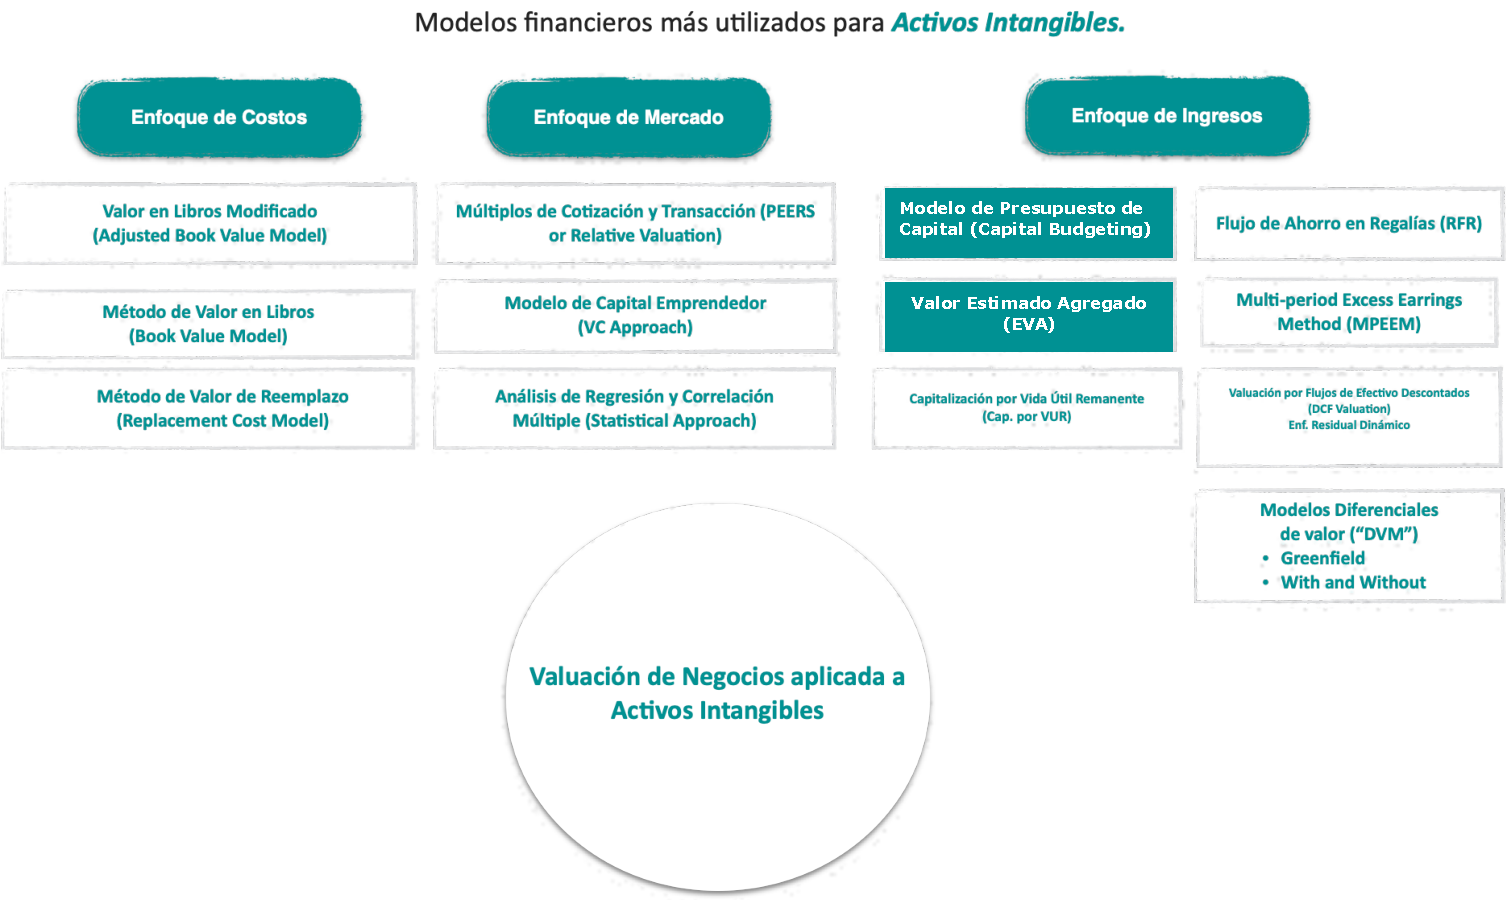
\includegraphics[width=17cm]{\rutaImagenes/metodologias_valuacion_intangibles_capital_budgeting_eva}\\

\end{figure}

\begin{enumerate}[1)]

\item \textbf{{\textprincipal}{Modelo de Presupuesto de Capital (Capital Budgeting).}}\\

Alcances y limitaciones del método:
\begin{itemize}

\item Los flujos de caja libres (FCL) deben medirse sobre una base posterior a los impuestos.
\item Todos los efectos indirectos de un proyecto, deben incluirse en los cálculos de un flujo de efectivo.
\item No deben considerarse los costos hundidos al evaluar un proyecto.
\item El valor de los recursos utilizados en un proyecto deben medirse en términos de sus costos de oportunidad.

\end{itemize}

La realización de dicha metodología requiere el cálculo de 2 premisas fundamentales:

\begin{figure}[H]
\centering
\caption{Elementos de la Inversión Neta:}
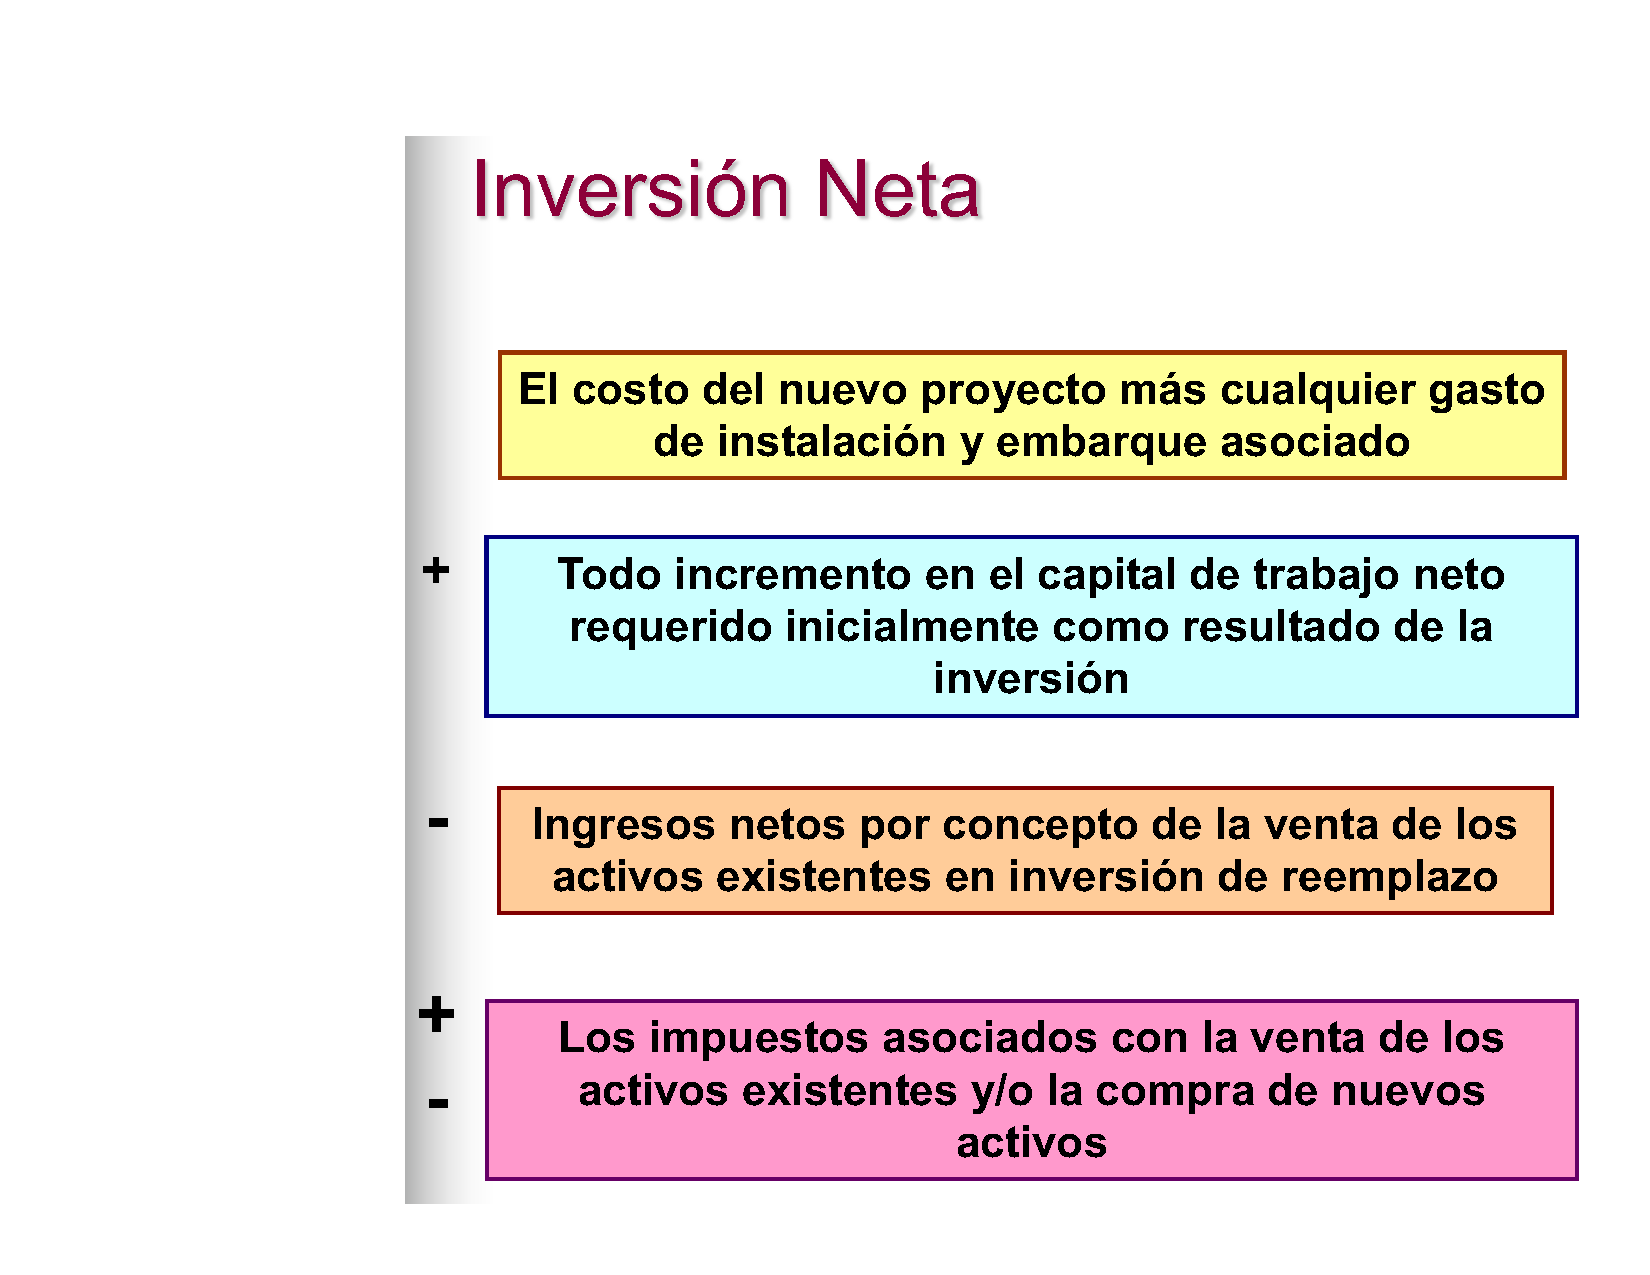
\includegraphics[width=8cm]{\rutaImagenes/CAPEX_1}\\
\end{figure}

\begin{figure}[H]
\centering
\caption{Estimación del Flujo de efectivo de operación neto:}
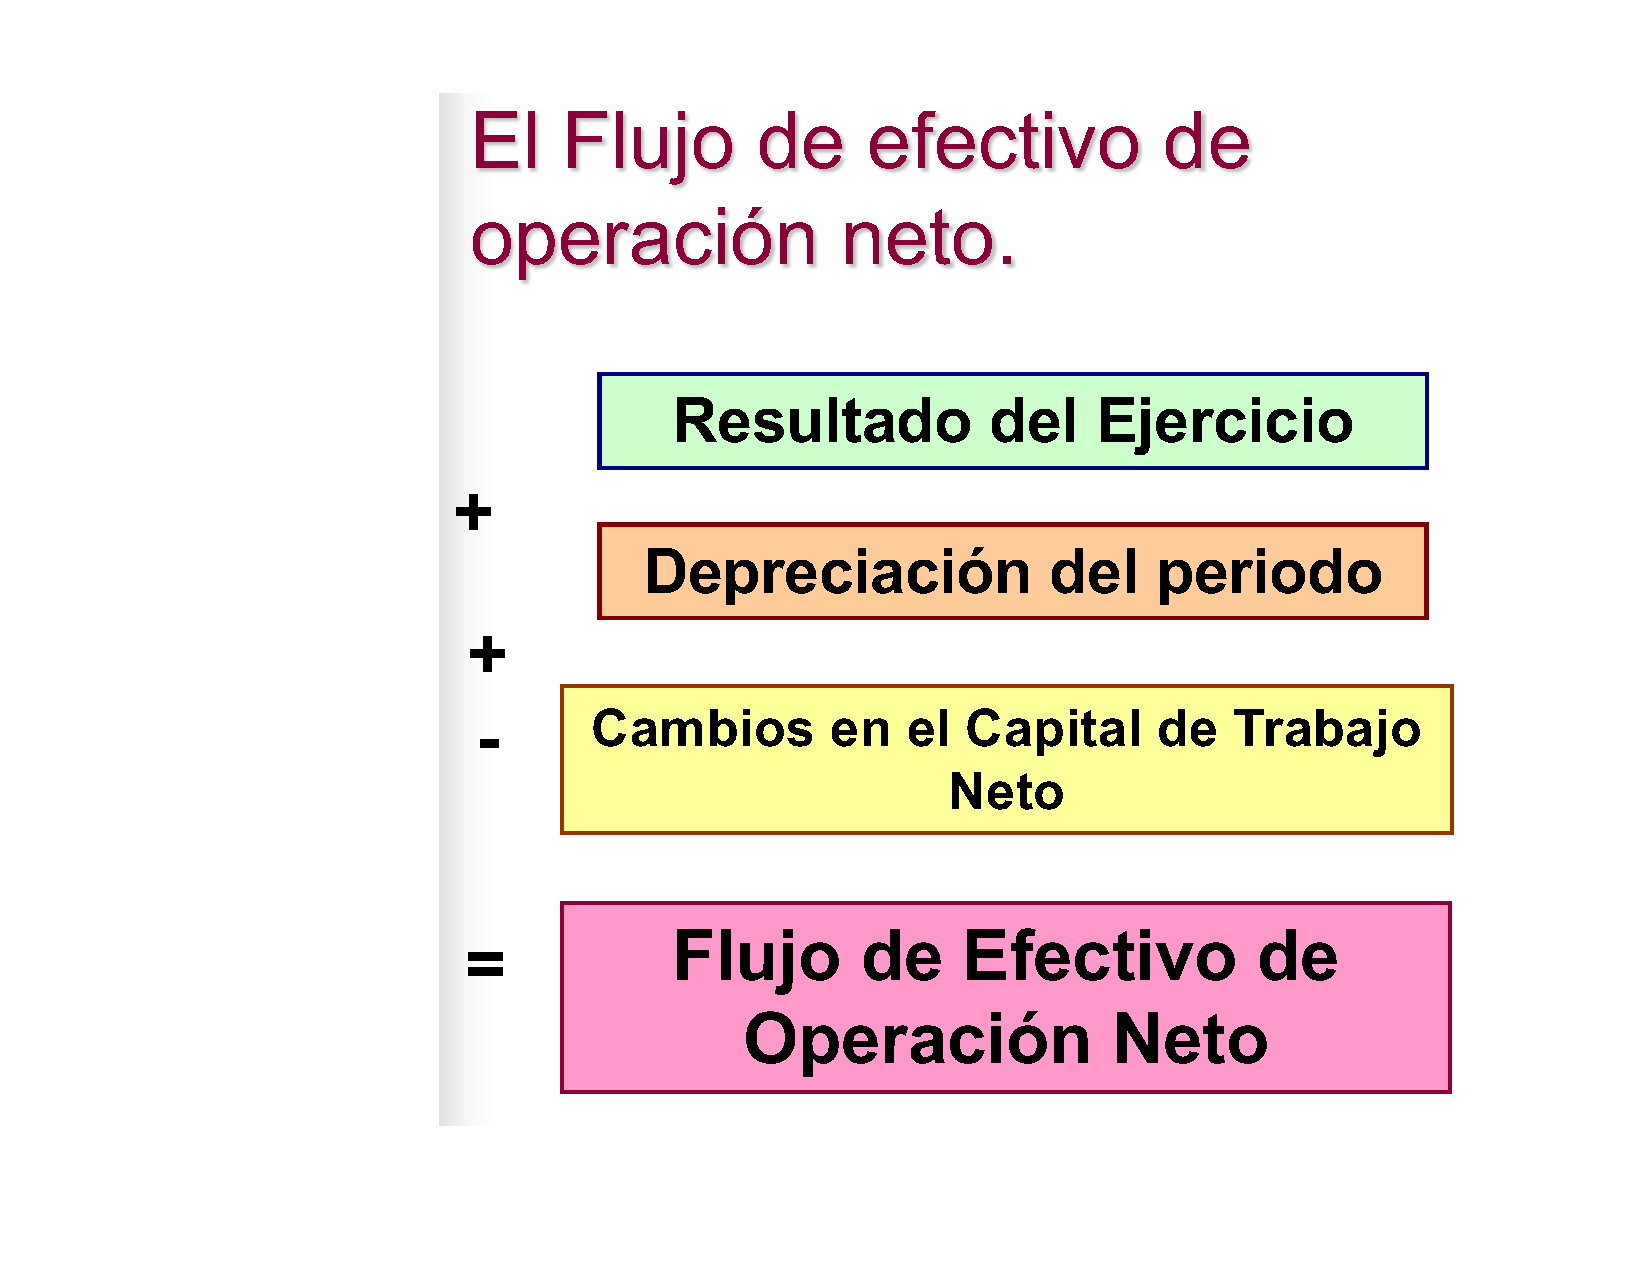
\includegraphics[width=8cm]{\rutaImagenes/CAPEX_2}\\
\end{figure}

\item Valor Agregado Estimado (EVA).

\begin{figure}[H]
\centering
\caption{Elementos de la Inversión Neta}
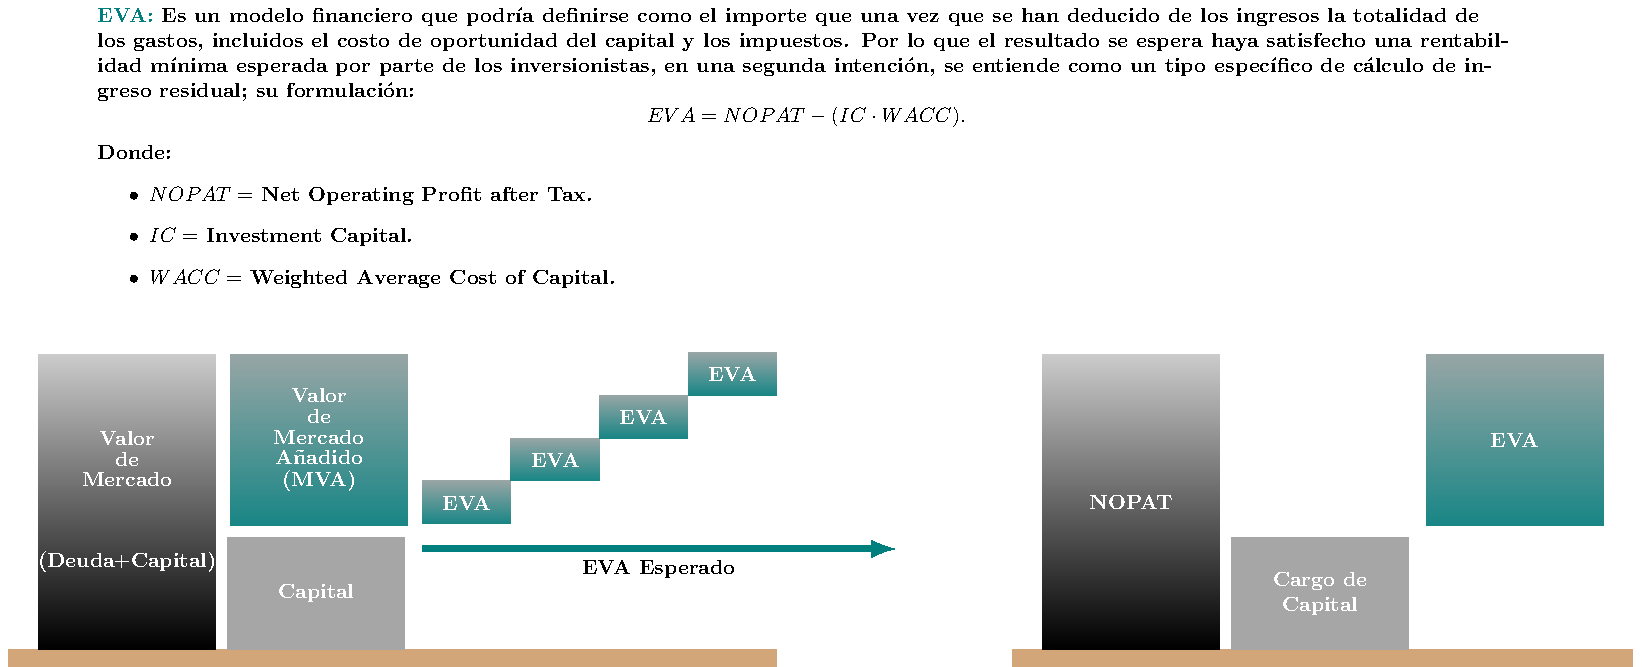
\includegraphics[width=\textwidth]{\rutaImagenes/eva}\\
\end{figure}


\end{enumerate}